\subsection*{a)}

\section*{Antwort}

S. Abbildung~\ref{fig:aufgabe-4-teil-a}.\\

\begin{figure}
    \centering
    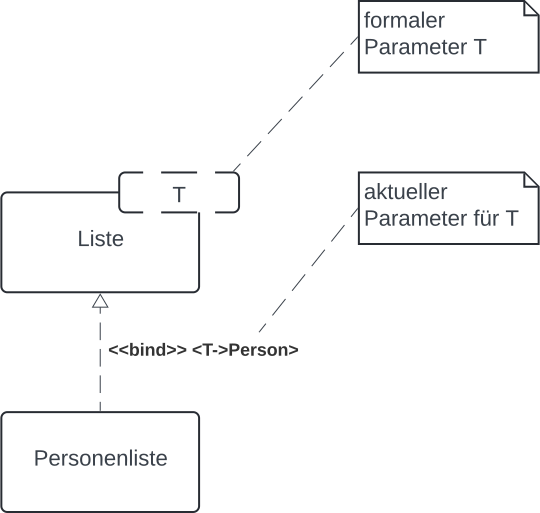
\includegraphics[scale=0.5]{chapters/aufgabe 4/img/aufgabe4a}
    \caption{Parametrisierte Klasse \textit{Liste} als Vorlage für die Klasse \textit{Personenliste}, die - der Bezeichnung der Klassen nach zu urteilen - Objekte vom Typ \textit{Person} verwaltet. (Quelle: eigene)}
    \label{fig:aufgabe-4-teil-a}
\end{figure}